\documentclass[tikz,border=8pt]{standalone}
% Shared look for every TikZ diagram. Load with \input{../../tools/tikz-style.tex}
\usepackage[T1]{fontenc}
\usepackage{lmodern}
\renewcommand{\sfdefault}{lmr}  % diagrams use the same serif as the text
\usetikzlibrary{arrows.meta, positioning, shapes.geometric, calc, fit, backgrounds}
\definecolor{cblue}{HTML}{4C78A8}
\definecolor{corange}{HTML}{F58518}
\definecolor{cgreen}{HTML}{54A24B}
\definecolor{cred}{HTML}{E45756}
\definecolor{cpurple}{HTML}{B279A2}
\definecolor{cgrey}{HTML}{6B6B6B}
\tikzset{
  every picture/.style={font=\sffamily, line width=1.2pt},
  box/.style={draw=#1, fill=#1!12, rounded corners=4pt, align=center, inner sep=7pt, minimum height=1.1cm},
  box/.default=cgrey,
  arrow/.style={-{Stealth[length=3mm]}, draw=cgrey, line width=1.4pt},
  title/.style={font=\sffamily\bfseries\Large},
  note/.style={font=\sffamily\small, text=cgrey, align=center},
}
\AtBeginDocument{\hyphenpenalty=10000 \exhyphenpenalty=10000}

\begin{document}
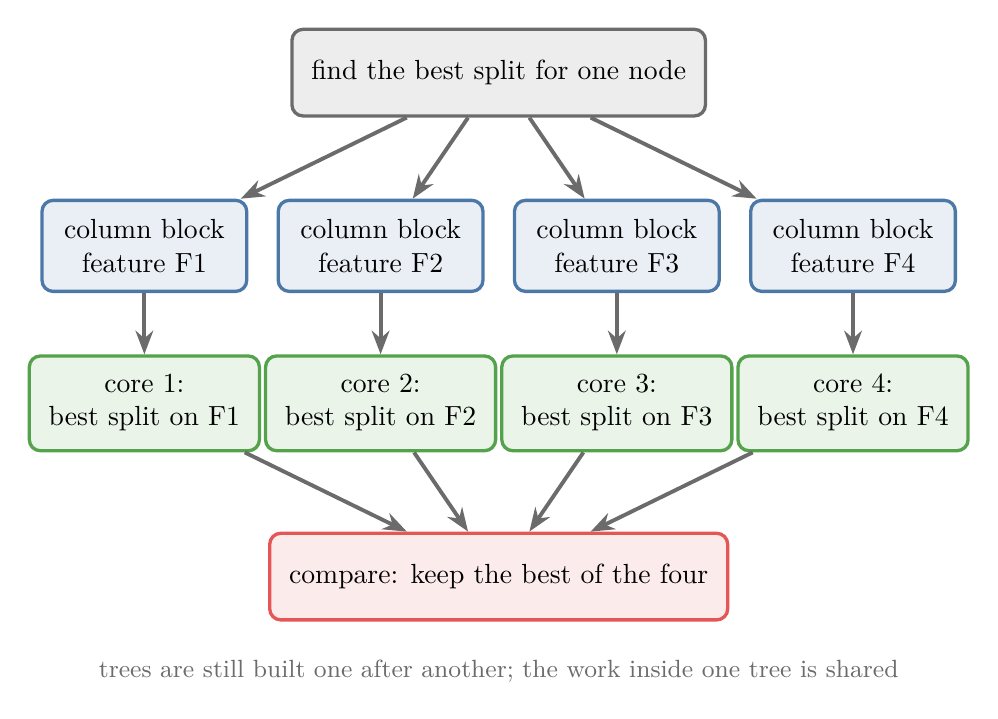
\begin{tikzpicture}[c/.style={box=cblue, minimum width=2.6cm}, g/.style={box=cgreen, minimum width=2.6cm}]
  \node[box=cgrey] (node) at (4.5,2.2) {find the best split for one node};
  \foreach \i/\x in {1/0,2/3,3/6,4/9} {
    \node[c] (f\i) at (\x,0) {column block\\feature F\i};
    \node[g] (k\i) at (\x,-2) {core \i:\\best split on F\i};
    \draw[arrow] (node) -- (f\i); \draw[arrow] (f\i) -- (k\i);
  }
  \node[box=cred, minimum width=5cm] (best) at (4.5,-4.2) {compare: keep the best of the four};
  \foreach \i in {1,...,4} {\draw[arrow] (k\i) -- (best);}
  \node[note] at (4.5,-5.4) {trees are still built one after another; the work inside one tree is shared};
\end{tikzpicture}
\end{document}
